\chapter{Theoretische Grundlagen} \label{chap:theoretische_grundlagen}  % Theorie
Zu Beginn dieser Studienarbeit werden die theoretischen Grundlagen erläutert, die für das Verständnis der späteren Kapitel notwendig sind. Dazu gehören die Funktionsweise von Machine Learning und Computer Vision, sowie die Grundlagen einer API.
Wie bereits im Ersten Kapitel (siehe Kapitel \ref{chap:problemstellung_und_ziel_dieser_arbeit}) beschrieben, baut diese Studienarbeit auf der Arbeit des letzten Semesters auf. 
Die theoretischen Grundlagen für Machine Learning und Computer Vision werden hier nut kurz erläutert, da sie bereits im letzten Semester ausführlich behandelt wurden.

Die Funktionsweise einer API wird in diesem Kapitel genauer erläutert, da sie eine zentrale Rolle in dieser Studienarbeit spielt. Mithilfe einer Web-API werden die Daten
des Python programmes an die entwickelte Webanwendung übertragen.

\section{Machine Learning und Klassifikationsprobleme} \label{sec:ml_cv}  % Theorie
Grundlegend, bevor die Datensätze in Form von Bildern durch Convoliutional Neural Networks \ac{CNN} analysiert werden können, müssen die Daten verarbeitet werden.

Bildverarbeitung beschäftigt sich mit der Manipulation und Analyse digitaler Bilder durch Algorithmen und bildet die Grundlage für komplexere Verfahren. 
Ein digitales Bild wird als mehrdimensionale Matrix gespeichert, wobei farbige Bilder als dreidimensionale Tensoren 
dargestellt werden, deren Dimensionen Höhe, Breite und Farbkanäle repräsentieren. 
Diese Repräsentation ermöglicht die Anwendung verschiedener Transformationen wie Filterung, Kontrastverbesserung oder geometrische Verzerrungen, die 
entweder zur Bildverbesserung oder als Vorverarbeitungsschritte für nachfolgende Analysen durch fortschrittlichere Techniken wie Machine Learning und Computer Vision dienen \cite{finbridgede_computer_2022}.

Convolutional Neural Networks \ac{CNN} sind spezialisierte Deep Learning Modelle, die für die Verarbeitung von Bilddaten optimiert sind. Sie bilden die Grundlage für zahlreiche moderne Computer Vision Anwendungen, wie Gesichtserkennung und autonome Fahrzeuge. 
Die Architektur eines CNN nutzt die räumliche Struktur von Bildern effizient, um visuelle Muster zu erkennen und zu klassifizieren.
Ein CNN besteht hauptsächlich aus Faltungsschichten und Linearen Ebenen (siehe \autoref{fig:system_overview}). 
Die Convolutional Layers verwenden kleine Filtermatrizen (Kernel), die über das Bild gleiten und visuelle Merkmale wie Kanten und Texturen erkennen. 
Diese Filter werden während des Trainings optimiert, um die relevantesten Merkmale zu extrahieren \cite{finbridgede_computer_2022} \cite{erfassung_convolutional_nodate}.

\begin{figure}[h]
    \centering
    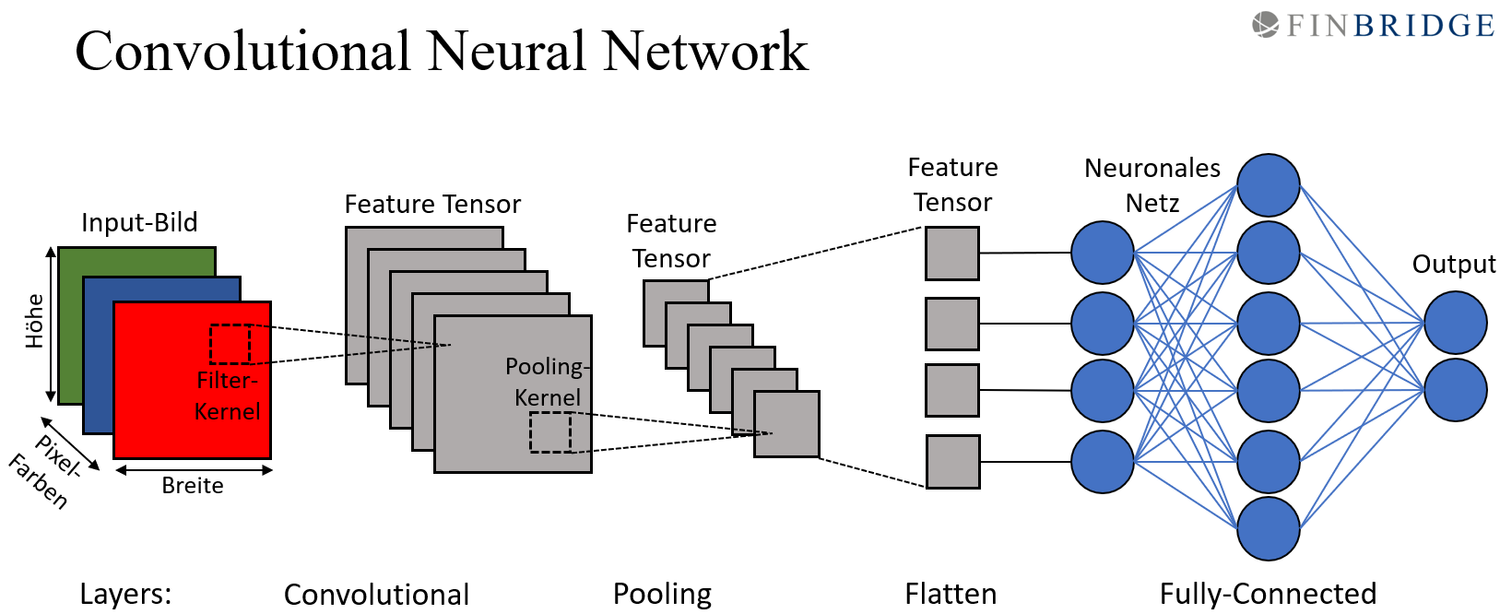
\includegraphics[width=1\textwidth]{CNN.png}
    \caption{Aufbau eines Convolutional Neural Networks \cite{finbridgede_computer_2022}.}
    \label{fig:system_overview}
\end{figure}

Die Fully-Connected Layers am Ende des Netzwerks (siehe \autoref{fig:system_overview}) wandeln die extrahierten Merkmale in eine endgültige Klassifikation oder Vorhersage um. Diese Schichten sind ähnlich wie traditionelle neuronale Netzwerke aufgebaut, wobei jedes Neuron mit allen Neuronen der vorherigen Schicht verbunden ist.

Die wichtigsten Lernansätze im maschinellen Lernen sind überwachtes, unüberwachtes und verstärkendes Lernen. In dieser Arbeit wird überwachtes Lernen genutzt, bei dem ein Algorithmus mit gelabelten Daten trainiert wird, um aus diesen Beispielen zu lernen und Vorhersagen zu treffen.

Beim überwachten Lernen gibt es zwei Hauptmodelle: Klassifikation und Regression. Regression beschreibt kontinuierliche Zusammenhänge zwischen Eingangs- und Ausgangsdaten \cite{noauthor_machine_nodate-1}. Klassifikation teilt Daten in diskrete Gruppen ein. Es sollen keine Kontinuierlichen werte nachgebildet werden. Am Ende des Netzwerks wird mithifge einer $argmax()$ Funktiion eine Klasse fest zugeordnet \cite[S. 450]{suse_bildverarbeitung_2014}. Die binäre Klassifikation, welche in dieser Arbeit angewandt wird ist eine spezielle Form der Klassifikation, bei der nur zwei Klassen unterschieden werden.

Es gibt verschiedene CNN-Architekturen wie ResNet und MobileNet, die für spezifische Aufgaben besonders gut geeignet sind. Oft werden vortrainierte Modelle verwendet und für spezifische Anwendungsfälle feinabgestimmt, eine Technik bekannt als Transfer Learning, welche auf dem überwachten Lernen basiert. \cite{finbridgede_computer_2022}.

\section{Die Funktionsweise einer API} \label{sec:api}  % Theorie

APIs stellen das Herzstück moderner Softwareentwicklung dar und ermöglichen es Programmen, miteinander zu kommunizieren und Daten auszutauschen. Dieser Datenaustausch ist wesentlich für vielfältige Anwendungen, wie etwa das Abrufen von Wetterdaten oder das Interagieren mit sozialen Netzwerken. In der Python Entwicklungsumgebung machen Bibliotheken wie requests oder http.client den Einstieg in die API-Entwicklung besonders zugänglich \cite{software_mittelstand_erste_nodate}. Die in dieser Studienarbeit verwendete FLASK Bibliothek ermöglicht es, eine komplextere API zu erstellen, die Daten aus dem Python Programm an die Webanwendung überträgt.

Anwendungsprogrammierschnittstellen \ac{API} sind Software-Vermittler; ihre Aufgabe besteht darin, Anwendungen die Kommunikation untereinander zu ermöglichen. Diese subtilen Vermittler sind allgegenwärtig im täglichen Leben, ob bewusst wahrgenommen oder nicht. Wenn man beispielsweise eine Sofortnachricht verschickt, nutzt man bereits eine \ac{API} \cite{pykes_programmieren_nodate}.

Im Kontext von Webanwendungen bieten \ac{API}s den Zugriff auf Daten und Funktionalitäten von Drittanbietern. Dies ermöglicht es Entwicklern, ihre Anwendungen um Funktionen wie Wetterinformationen, Sportergebnisse, Filmlisten, Tweets, Suchmaschinenergebnisse und Bildverarbeitung zu erweitern. Zudem können über APIs weitere Funktionalitäten wie Zahlungsabwicklung, Terminplanung, E-Mail-Versand, Übersetzungen, Kartendienste oder Dateiübertragungen integriert werden. Die Eigenentwicklung solcher Funktionen würde erhebliche Ressourcen beanspruchen, während die Nutzung von APIs eine schnelle und effiziente Integration ermöglicht\cite{digital_ocean_llc_erste_nodate}.


\subsection{Anfragearten einer API} \label{subsec:anfragearten_einer_api}  % Theorie

\subsection{FLASK} \label{subsec:flask}  % Theorie